
\documentclass[12pt,halfline,a4paper,]{ouparticle}

% Packages I think are necessary for basic Rmarkdown functionality
\usepackage{hyperref}
\usepackage{graphicx}
\usepackage{listings}
\usepackage{xcolor}
\usepackage{fancyvrb}
\usepackage{framed}

% Link coloring
\hypersetup{breaklinks=true,
            bookmarks=true,
            pdfauthor={},
            pdftitle={STA2005S - Regression Assignment}
            }


%% To allow better options for figure placement
%\usepackage{float}

% Packages that are supposedly required by OUP sty file
\usepackage{amssymb, amsmath, geometry, amsfonts, verbatim, endnotes, setspace}

% use upquote if available, for straight quotes in verbatim environments
\IfFileExists{upquote.sty}{\usepackage{upquote}}{}

% Macros for dealing with affiliations, footnotes, etc.
\makeatletter
\def\Newlabel#1#2#3{\expandafter\gdef\csname #1@#2\endcsname{#3}}

\def\Ref#1#2{\@ifundefined{#1@#2}{???}{\csname #1@#2\endcsname}}

\newcommand*\samethanks[1][\value{footnote}]{\footnotemark[#1]}

\newcommand*\ifcounter[1]{%
  \ifcsname c@#1\endcsname
    \expandafter\@firstoftwo
  \else
    \expandafter\@secondoftwo
  \fi
}

\newcommand*\thanksbycode[1]{%
  \ifcounter{FNCT@#1}
    {\samethanks[\value{FNCT@#1}]}
    {\thanks{\Ref{FN}{#1}}\newcounter{FNCT@#1}\setcounter{FNCT@#1}{\value{footnote}}}
}

% Create labels for Addresses if the are given in Elsevier format

% Create labels for Footnotes if the are given in Elsevier format

% Part for setting citation format package: natbib

% Part for setting citation format package: biblatex


% tightlist command for lists without linebreak
\providecommand{\tightlist}{%
  \setlength{\itemsep}{0pt}\setlength{\parskip}{0pt}}



\usepackage{float} \floatplacement{figure}{H} \usepackage{caption} \captionsetup[figure]{font=scriptsize} \renewenvironment{abstract}{}{} \renewenvironment{keywords}{}{}

\begin{document}

\title{STA2005S - Regression Assignment}

\author{%
%
% Code for old style authors field
%
% Add \and if both authors and author
%
%
% Code for new (elsevier) style author field
\name{Jing Yeh}
%
\email{\href{mailto:yhxjin001@myuct.ac.za}{yhxjin001@myuct.ac.za}}%
%
%
%
\and
\name{Saurav Sathnarayan}
%
\email{\href{mailto:sthsau001@myuct.ac.za}{sthsau001@myuct.ac.za}}%
%
%
%
%
}

\abstract{}

\date{2024-10-13}

\keywords{}

\maketitle



\newpage

\hypertarget{part-one-analysis}{%
\subsection{Part One : Analysis}\label{part-one-analysis}}

\hypertarget{section-1-introduction}{%
\section{Section 1: Introduction}\label{section-1-introduction}}

Air pollution, particularly high levels of particulate matter (PM), is a
major environmental and public health issue in South Africa's urban
centers. Exposure to elevated PM levels is linked to respiratory
diseases and other serious health conditions. Understanding the factors
influencing PM concentrations is crucial for developing policies that
improve air quality and protect public health. This analysis seeks to
identify the key drivers of air pollution in South Africa's cities,
focusing on how various urban, environmental, and socioeconomic factors
affect particulate matter levels.\\
Unknown Factors to Investigate:\\
Traffic Density: How do varying levels of vehicle traffic contribute to
PM levels in different areas?\\
Industrial Activity: What is the impact of industrial activity near
monitoring stations on air quality?\\
Temperature \& Humidity: How do changes in weather conditions, like
temperature and humidity, influence PM concentrations?\\
Wind Speed: How does wind speed affect the dispersion or accumulation of
particulate matter in urban areas?\\
Day of the Week \& Public Holidays: Do patterns of human activity on
weekdays, weekends, and holidays significantly influence pollution
levels?\\
Urban Greenery: How effective are green spaces in reducing air pollution
in densely populated areas?\\
\# Objective\\
The goal of this analysis is to explore the relationships between PM
levels and these explanatory variables. By identifying the most
influential factors, we aim to inform urban planning and public health
strategies that address air pollution and improve the quality of life in
South African cities.

\hypertarget{including-plots}{%
\subsection{Including Plots}\label{including-plots}}

You can also embed plots, for example:

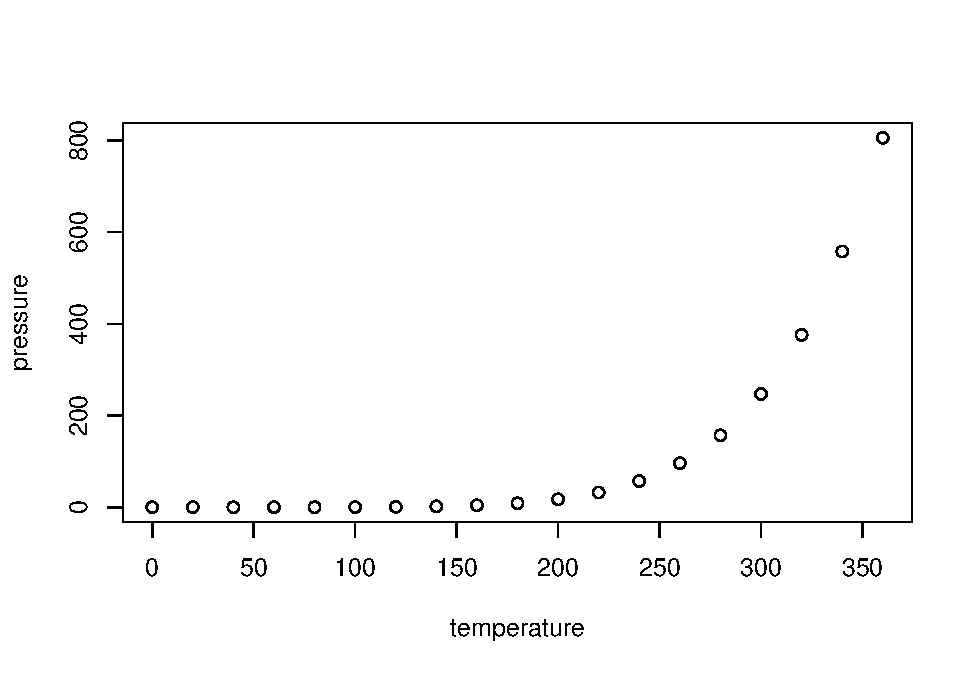
\includegraphics{Report_files/figure-latex/pressure-1.pdf}

Note that the \texttt{echo\ =\ FALSE} parameter was added to the code
chunk to prevent printing of the R code that generated the plot.






\end{document}
